\documentclass{beamer}
\usetheme{ConnectivityLab}
\usepackage{times}
\usepackage{graphicx}
\usepackage{verbatim}
\usepackage{outlines}
\usepackage{fancyhdr}
\usepackage{subfigure}
\usepackage{cancel}
\usepackage{bibentry}
\usepackage{varwidth}
\usepackage{etoolbox}
\usepackage{epstopdf}

%%%%%%%%%%%%%%%%%%%%%%%%%%%%%%%%%%%%%%%%%%%%%%%%%%%%%%
%%%%%%%%%%%%%%%%%%%%%%%%%%%%%%%%%%%%%%%%%%%%%%%%%%%%%%

\title {
    Progress Report
}
\author {
    Yin-Hong Hsu
}
\date {
    03 23, 2018
}

%%%%%%%%%%%%%%%%%%%%%%%%%%%%%%%%%%%%%%%%%%%%%%%%%%%%%%
%%%%%%%%%%%%%%%%%%%%%%%%%%%%%%%%%%%%%%%%%%%%%%%%%%%%%%

\begin{document}
\begin{frame}
    \titlepage
\end{frame}

%%%%%%%%%%%%%%%%%%%%%%%%%%%%%%%%%%%%%%%%%%%%%%%%%%%%%%
%%%%%%%%%%%%%%%%%%%%%%%%%%%%%%%%%%%%%%%%%%%%%%%%%%%%%%

\begin{frame}{Outline}
    \tableofcontentsgather
    \tableofcontents
\end{frame}

%%%%%%%%%%%%%%%%%%%%%%%%%%%%%%%%%%%%%%%%%%%%%%%%%%%%%%
%%%%%%%%%%%%%%%%%%%%%%%%%%%%%%%%%%%%%%%%%%%%%%%%%%%%%%
\section{Progress}
\begin{frame}{}
    \begin{itemize}
        \item {Mobile Crowd Sensing (MCS) framework.}
        \item {Data Collection Element (Fog node) will verify the signature and do message pre-processing.}
        \item {While Mobile User (MU) leave from BS1 to BS2, BS2 will notify Key Authority to move MU's public key from ring1 to ring2.}
    \end{itemize}
\end{frame}
\begin{frame}{}
    \begin{figure}[t]
        \centering
        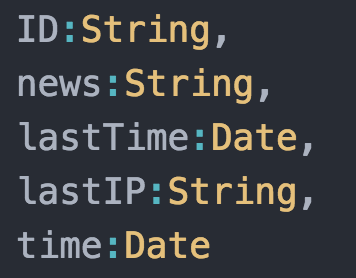
\includegraphics[width=1.0\textwidth]{figures/1.png}
        \setbeamerfont{caption}{size=\tiny}
        \caption{Architecture}
    \end{figure}
\end{frame}
\begin{frame}{}
    \begin{figure}[t]
        \centering
        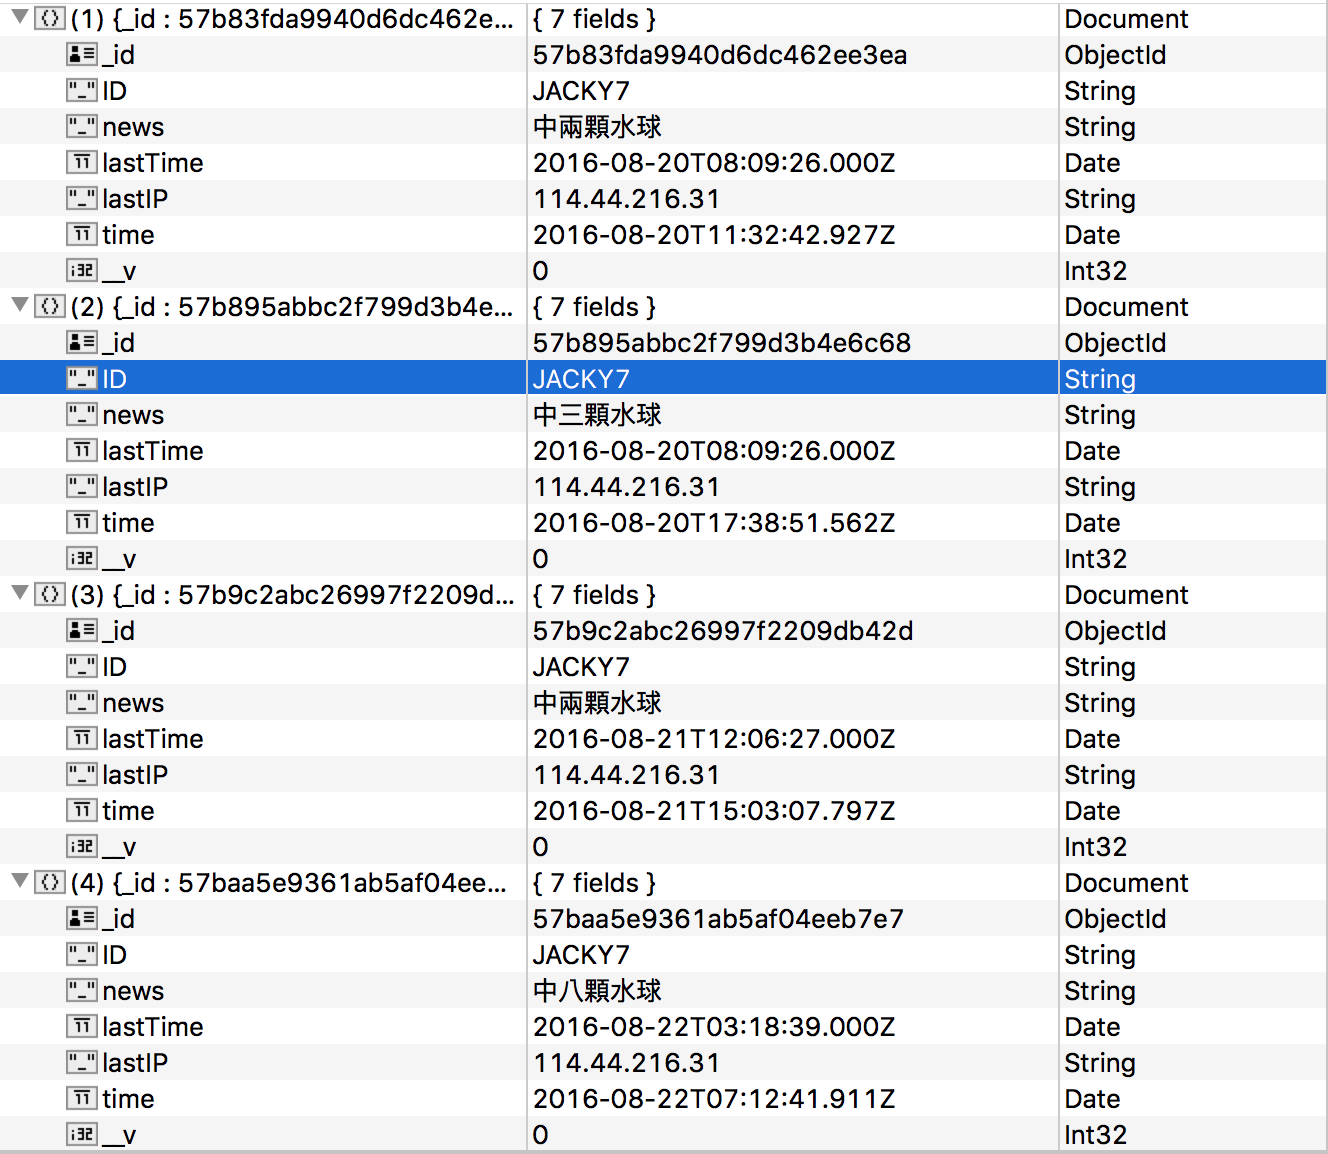
\includegraphics[width=1.0\textwidth]{figures/2.png}
        \setbeamerfont{caption}{size=\tiny}
        \caption{Security Process}
    \end{figure}
\end{frame}
\begin{frame}{}
    \begin{figure}[t]
        \centering
        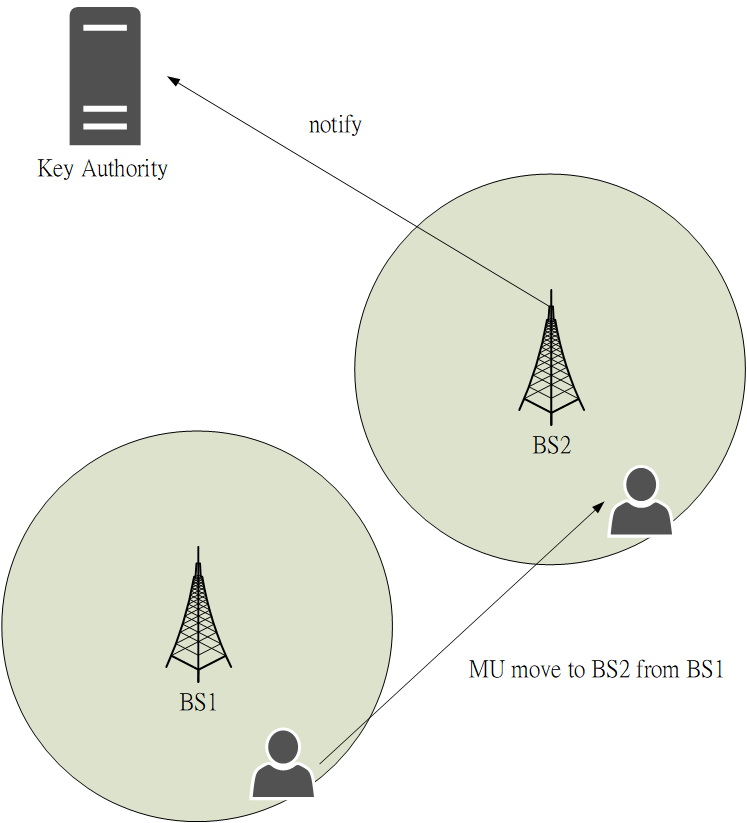
\includegraphics[width=0.7\textwidth]{figures/3.png}
        \setbeamerfont{caption}{size=\tiny}
        \caption{leave, join}
    \end{figure}
\end{frame}
%%%%%%%%%%%%%%%%%%%%%%%%%%%%%%%%%%%%%%%%%%%%%%%%%%%%%%
%%%%%%%%%%%%%%%%%%%%%%%%%%%%%%%%%%%%%%%%%%%%%%%%%%%%%%

\section{References}
\calcreferencespagetotal % Calc your References Page total number
\begin{frame}[allowframebreaks]{References}
    \fontsize{9pt}{13}\selectfont
    \bibliographystyle{IEEEtran}
    \bibliography{IEEEabrv,Citation}
\end{frame}

%%%%%%%%%%%%%%%%%%%%%%%%%%%%%%%%%%%%%%%%%%%%%%%%%%%%%%
%%%%%%%%%%%%%%%%%%%%%%%%%%%%%%%%%%%%%%%%%%%%%%%%%%%%%%
\section{}

\begin{frame}
    \centering
    \Large{Thanks for Your Attentions}
\end{frame}

\end{document}
